\documentclass{standalone}
\usepackage{tikz}
\begin{document}
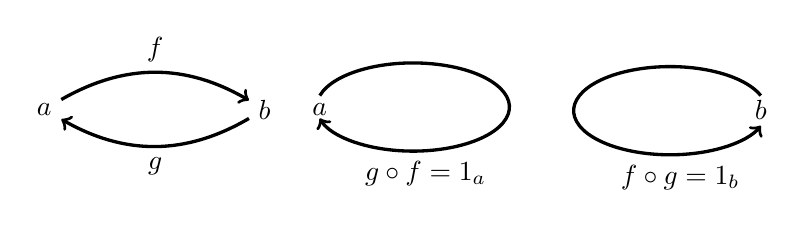
\begin{tikzpicture}[scale=0.7]
    \tikzset{arc lines/.style={very thick,black, ->}}
    % \draw (0, 0) grid (16, 2);

    \node (0) at (5, 0) {$a$};
    \node (1) at (5, 0.25) {};
    \draw[arc lines] (1) arc [start angle=15, end angle=345, x radius=-1.75cm, y
        radius=0.8cm]
        node[pos=0.75, below] {$g\circ f=1_a$}
        ;
    \node (0) at (13, 0) {$b$};
    \node (1) at (13, 0.25) {};
    \draw[arc lines] (1) arc [start angle=20, end angle=340, x radius=1.75cm, y
        radius=0.8cm]
        node[pos=0.8, below] {$f\circ g=1_b$}
        ;
    \node (0) at (0, 0) {$a$};
    \node (1) at (4, 0) {$b$};
    \draw [arc lines, ->, bend left=30] (0) to node[pos=0.5, above] {$f$} (1);
    \draw [arc lines, ->, bend left=30] (1) to node[pos=0.5, below] {$g$} (0);
\end{tikzpicture}
\end{document}
